\documentclass[12pt]{article}
\usepackage{amsmath}
\usepackage[shortlabels]{enumitem}
\usepackage{tcolorbox}

\usepackage{graphicx}
\usepackage{amsthm}
\usepackage{amssymb}
\usepackage{thmtools}
\usepackage{amsthm}
\usepackage{algorithm}
\usepackage{algpseudocode}
\usepackage{xspace}
\usepackage{CJKutf8}
\usepackage[hidelinks,pdfencoding=auto,psdextra]{hyperref}

\usepackage{graphicx}
\usepackage{pythonhighlight}


%\renewcommand{\thepage}{}

\textwidth=6.7in
\textheight=8.4in
\oddsidemargin=-.3in
\evensidemargin=-.1in
\topmargin=-.3in

\newcommand{\Bskip}{\vspace*{.3in}}
\newcommand{\Solution}{\ \\ \textbf{Solution:} }
\newcommand{\Answer}{\ \\ \textbf{Answer:} }
\newtheorem{theorem}{Theorem}
\newtheorem{remark}{Remark}
\newtheorem{hint}{Hint}
\newtheorem{definition}{Definition}

\DeclareMathOperator*{\E}{\mathbb{E}}
\newcommand{\Var}{\mathsf{Var}}
\newcommand{\Cov}{\mathsf{Cov}}
\newcommand{\Covar}{\mathsf{Covar}}
\declaretheoremstyle[headfont=\bf]{normalhead}
\declaretheorem[style=normalhead]{problem}
\def\ie{\textit{i.e.}\xspace}
\def\eg{\textit{e.g.}\xspace}
\newcommand{\Name}{Jin Fang}
\newcommand{\ChineseName}{方缙}

\begin{document}

\noindent
\hspace*{.2in} COMP7102P Fall 2022
\hfill Homework 2\\
\begin{CJK}{UTF8}{gbsn}
    \hspace*{.2in} \textcolor{red}{BA22011024 \Name{} \ChineseName} \hfill due: Oct. 27, 09:30
\end{CJK}
\bigskip


\begin{problem}[30 points] Answer the following questions and show your calculations.
\begin{enumerate}
  \item Compute the stationary distribution of the standard random walk (pick a random outgoing edge and traverse along this edge) for the following directed graph.
 \begin{figure}[H]
      \centering
 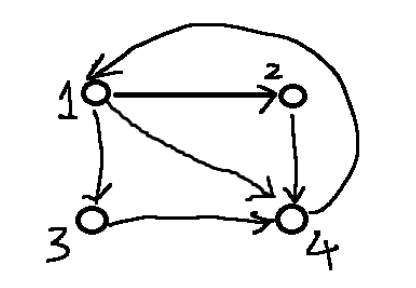
\includegraphics[width=2in]{images/123.png}
\end{figure}     
   Remark: Unlike undirected graphs whose stationary distributions have a close form, there is no close form for directed graph.
   
  \Answer
  The transition matrix $A$ of the following directed graph is 
  \begin{equation}
  A = {
\left( \begin{array}{cccc}
0 & \frac{1}{3} & \frac{1}{3} & \frac{1}{3}\\
0 & 0 & 0 & 1\\
0 & 0 & 0 & 1 \\
1 & 0 & 0 & 0 
\end{array}
\right )}.
  \end{equation}
 Assume the stationary distribution is $\mathbf{\pi} = (\pi_1, \pi_2, \pi_3, \pi_4)$. We have $\mathbf{\pi}A = \mathbf{\pi}$, that is,
\begin{align}\label{5}
\begin{cases}
\pi_4 = \pi_1\\
 \frac{\pi_1}{3} = \pi_2\\
  \frac{\pi_1}{3} = \pi_3\\
  \frac{\pi_1}{3}+\pi_2+\pi_3 = \pi_4\\
  \pi_1+ \pi_2+ \pi_3+ \pi_4 =1
\end{cases}
\end{align}
 By solving Eq .\eqref{5}, we obtain,
 \begin{align}
\begin{cases}
 \pi_1 = \frac{3}{8}\\
 \pi_2 = \frac{1}{8}\\
 \pi_3 = \frac{1}{8}\\
 \pi_4 = \frac{3}{8}
\end{cases},
\end{align}
the stationary distribution is $\mathbf{\pi} = (\frac{3}{8}, \frac{1}{8},\frac{1}{8}, \frac{3}{8})$.
      
  \item Consider a start graph with $n$ vertices. Suppose vertex 1 is the center. What are the hitting time $h_{1,2}$ and $h_{2,1}$?
   \begin{figure}[H]
      \centering
 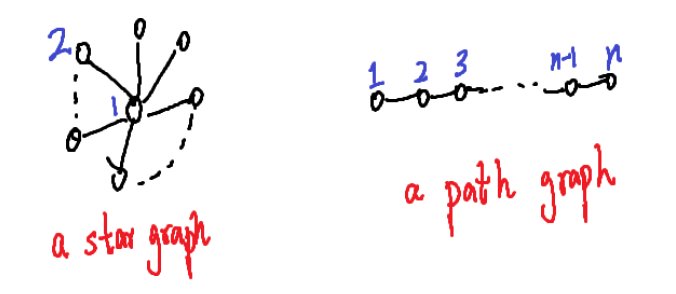
\includegraphics[width=4in]{images/1234.png}
\end{figure} 
  
  \Answer
  For the star graph, we have
  \begin{align}\label{7}
\begin{cases}
h_{1,2} = \sum_{i=3}^{n}\frac{1+h_{i,2}}{n-1} + \frac{1}{n-1}\\
h_{3,2} = 1+h_1,2\\
\cdots\\
h_{n,2} = 1+h_1,2\\
\end{cases}
\end{align}
  By Eq. \eqref{7}, we derive
  \begin{align}
  &  h_{1,2} = (n-2)\frac{2+h_{1,2}}{n-1} + \frac{1}{n-1}\nonumber\\
   \Longrightarrow &(n-1) h_{1,2} =  (n-2)(2+h_{1,2}) +1\nonumber\\
   \Longrightarrow&  h_{1,2} = 2n-3  
  \end{align}
  Therefore, we have $h_{1,2} = 2n-3$. Apparently,  $h_{2,1} = 1$.
  
  \item Consider a path graph with from 1 to n. What are the hitting time $h_{1,n}$ and $h_{n,1}$?
    \Answer
    For the linear graph, we have
  \begin{align}\label{10}
\begin{cases}
h_{1,n} = 1+h_{2,n} \\
h_{2,n} =1+ \frac{1}{2}(h_{1,n}+h_{3,n})\\
h_{3,n} =1+ \frac{1}{2}(h_{2,n}+h_{4,n})\\
h_{4,n} =1+ \frac{1}{2}(h_{3,n}+h_{5,n})\\
\cdots\\
h_{n-2,n} =1+ \frac{1}{2}(h_{n-1,n}+h_{n-3,n})\\
h_{n-1,n} =1+ \frac{1}{2}h_{n-2,n}.
\end{cases}
\end{align}
  By adding the left and right sides of Eq. \eqref{10} respectively, we get
  \begin{align}
  &  h_{1,n}+h_{2,n}+h_{n-1,n} = n-1 + \frac{3}{2}h_{2,n} +\frac{1}{2}h_{1,n}+\frac{1}{2}h_{n-1,n} \nonumber\\
   \Longrightarrow &h_{n-1,n} = 2n-3
  \end{align}
  By using $h_{n-1,n} = 2n-3$, we recursively solve Eq. \eqref{10} as follows,
  \begin{align}\label{15}
\begin{cases}
h_{n-1,n} = 2n-3 \\
h_{n-2,n} =4n-8\\
h_{n-3,n} =6n-15\\
\cdots\\
h_{n-i,n} =2ni - i(i+2)\\
\cdots\\
h_{2,n} =n(n-2)\\
h_{1,n} =n(n-2)+1.
\end{cases}
\end{align}
As a result, we obtain that $h_{1,n} =n(n-2)+1$. Similarly, we can derive that $h_{n,1} =n(n-2)+1$, too.
  
  
\end{enumerate}

\end{problem}

\begin{problem}[40 points] Let us compute the mixing time by a different way. Let $A$ be the transition matrix of a undirected graph $G: A(i, j) = 1/d(i) \text{\ iff\ }(i, j) \in E$. Let $A = \sum_{i=1}^{n}\lambda_i\cdot D^{-1/2}\mathop{v_{i}}\limits ^{\rightarrow}\cdot D^{-1/2}{\mathop{v_{i}}\limits ^{\rightarrow}}^\top$ be its eigen-decomposition where $\mathop{v_{1}}\limits ^{\rightarrow},\mathop{v_{2}}\limits ^{\rightarrow},...,\mathop{v_{n}}\limits ^{\rightarrow}$ constitute an orthonormal basis.
\end{problem}
\begin{enumerate}
	\item Write all facts that we have shown about $\lambda_1,...,\lambda_n$ and $\mathop{u_{1}}\limits^{\rightarrow}$.
	\item Let $p_0$ be the distribution of the starting point of our random walk. Prove $p_t^\top=p_0^\top\cdot A^t$ and $||p_t - \pi||_2 \le \max\{\lambda_2,|\lambda_n|\}\cdot||p_{t-1}-\pi||_2$.
	\item Conclude that for $t\ge\frac{10\log{\frac{n}{\epsilon}}}{1-\max\{\lambda_2,|\lambda_n|\}}$,$||p_t-\pi||_1\le\epsilon$ (note that we switch to $\ell_1$ norm here).
\end{enumerate}

\begin{problem}[30 points] Consider the Boolean cube $B_n$ of dimension $n: V=\{0,1\}^n$ and $E=\{(x,y)\}$ where the difference between $x$ and $y$ is just 1 bit. See Figure 3 for $B_3$.
\end{problem}
\begin{figure}[H]
	\centering
	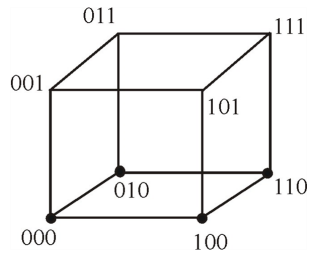
\includegraphics[width=2in]{images/p2.png}\\
	Figure 3: Boolean cube of dimension 3
\end{figure} 
\begin{enumerate}
	\item Compute the eigenvalues and eigenvectors of $B_n$.
	\item Consider lazy random walk where we stay at the current vertex with probability .5 and move along an edge with probability .5. Bound the mixing time of lazy random walk in	$B_n$ by eigenvalues.
	
  \Answer
	Let $N$ be the transition matrix of random walk on the cube $B_n$. Then we know that: $N = 1 \cdot Q_n$. For the matrix $N$, denote its eigenvalues by $\eta$, we have: $\eta_i = \frac{1}{n} \cdot \lambda_i$. And we know that the stationary distribution of the random walk on the cube is just like that in the lecture, with $2^n$ vertices in the graph. So its stationary distribution
  $\pi(j)=\frac{deg(j)}{|E|}= \frac{n}{n \cdot 2^n}=\frac{1}{2^n}$.

  Now we consider the lazy random walk. Its transition matrix $A= \frac{1}{2} \cdot I + \frac{1}{2} \cdot N$, so its eigenvalues(denoted by $\mu$) $\mu_i = \frac{1}{2} + \frac{1}{2} \cdot \mu_i =\frac{1}{2} + \frac{1}{2 \cdot n}\lambda_i$, and its stationary distribution is the same with the ordinary random walk. From part 1 of this problem, we can see that $\lambda \in [-n, n]$, so we have:

  \begin{equation}
    1 = \mu_1 \geq \dots \geq \mu_{2^n} \geq 0
  \end{equation}
  
  Denote the eigenvectors of $A$ by $v$. We have:

  \begin{align}
    v_1 &= (\sqrt{\frac{d_1}{2m}}, \dots, \sqrt{\frac{d_n}{2m}})^T \\
    &=(\sqrt{\frac{1}{2^n}}, \dots, \sqrt{\frac{1}{2^n}})^T
  \end{align}

  Because $A$ is symmetric, we have:

  \begin{align}
    A = \sum\limits_{i=1}^{2^n} \mu_i \cdot \overrightarrow{v_i} \cdot \overrightarrow{v_i}^T
  \end{align}

  So we have:
  
  \begin{align}
    p_t^T &= p_0^T \cdot A^t \\
    &= p_0^T \cdot \sum\limits_{i=1}^{2^n} \mu_i^t \cdot \overrightarrow{v_i} \cdot \overrightarrow{v_i}^T
  \end{align}

  So 

  \begin{align}
    p_t(j) &= \sum\limits_{i=1}^{2^n} p_0(i) \cdot A^t(i,j) \\
    &= \sum\limits_{i=1}^{2^n} p_0(i) \cdot [\pi(i)+ \sum\limits_{k=2}^{2^n}\mu_k^tv_k(i)v_k(j)] \\
    &= \pi(j)+\sum_{i=1}^{2^n} p_0(i) \cdot [\sum\limits_{k=2}^{2^n}\mu_k^tv_k(i)v_k(j)]
  \end{align}

  We have:

  \begin{align}
    |p_t-\pi|_{1} &= \sum\limits_{j=1}^{2^n} |p_t(j) - \pi(j)| \\
    &= \sum\limits_{i=1}^{2^n} |\sum\limits_{j=1}^{2^n} (p_0(i) \cdot \sum\limits_{k=2}^{2^n} \mu_k^tv_k(i)v_k(j) | \\
    &\leq \sum\limits_{j=1}^{2^n} |2^n \cdot \max\limits_{k=2 \backsim 2^n} \mu_k^t \\
    & \leq 2^{2n} \cdot |\mu_2^t
  \end{align}

  \item Argue that it takes $\Omega(n\log n)$ time to mix in expectation.
\end{enumerate}
\end{document}
